\documentclass[letterpaper]{article}
\usepackage[submission]{aaai2027}
\usepackage[hyphens]{url}
\usepackage{graphicx}
\urlstyle{rm}
\def\UrlFont{\rm}
\usepackage{natbib}
\usepackage{caption}
\usepackage{booktabs}
\usepackage{xcolor}
\newcommand{\shadedrow}{\rlap{\color{gray!18}\rule[-3pt]{\dimexpr\textwidth\relax}{10pt}}}
\usepackage{float}
\floatstyle{ruled}
\newfloat{algorithm}{t}{alg}
\floatname{algorithm}{Algorithm}
\usepackage{dcolumn}
\usepackage{amsmath}
\newcolumntype{d}{D{.}{.}{-1}}
\frenchspacing

\pdfinfo{
/TemplateVersion (2027.1)
}

\setcounter{secnumdepth}{1}

\title{When Common Sense Overrides Vision:\\Diagnosing and Correcting Directed Prior Attraction}
\author{Anonymous Submission}
\affiliations{}

\begin{document}
\maketitle

\begin{abstract}
Commonsense-driven hallucination (CDH) occurs when a vision--language model
replaces atypical visual evidence with the ordinary state it expects such as six-finger hand. 
These errors have a destination: when the model fails on a counterfactual
image, its wrong answer is usually the exact answer favored by its own
text-only prior, and matched commonsense controls show that this same prior is
often useful. Methods that broadly suppress language priors can therefore trade
one failure for another. We introduce Candidate-Aligned Prior-Residual Calibration
(CPRC), which scores the native answer candidates with and without the image,
learns from a small set of paired examples how strongly to subtract each
candidate's prior preference, and keeps the native answer unless the score
pattern supports a change. On unseen concepts and independent conflict
benchmarks, CPRC recovers substantial counterfactual accuracy while leaving
commonsense behavior nearly intact; calibrated separately for each model, the
method generalizes across semantic families, answer permutations, and datasets,
and replicates across model architectures. On
benchmarks without CDH-type conflicts, CPRC changes almost no answers, with no
significant accuracy loss. CDH thus emerges as a correctable error
with a measurable scope: the calibration intervenes where world knowledge
overrides vision and largely preserves native behavior elsewhere.
\end{abstract}

\section{Introduction}

Consider the same question asked about two images: ``How many heads does the
dog have?'' The ordinary dog has one head and the model answers one. The
counterfactual dog visibly has two, yet the model again answers one. The queried
object is present, the relevant evidence is visible, and the answer vocabulary
is unchanged. Only the relationship between seeing and knowing has reversed:
visual evidence supports two, while ordinary-world knowledge favors one.

\begin{figure*}[t]
\centering
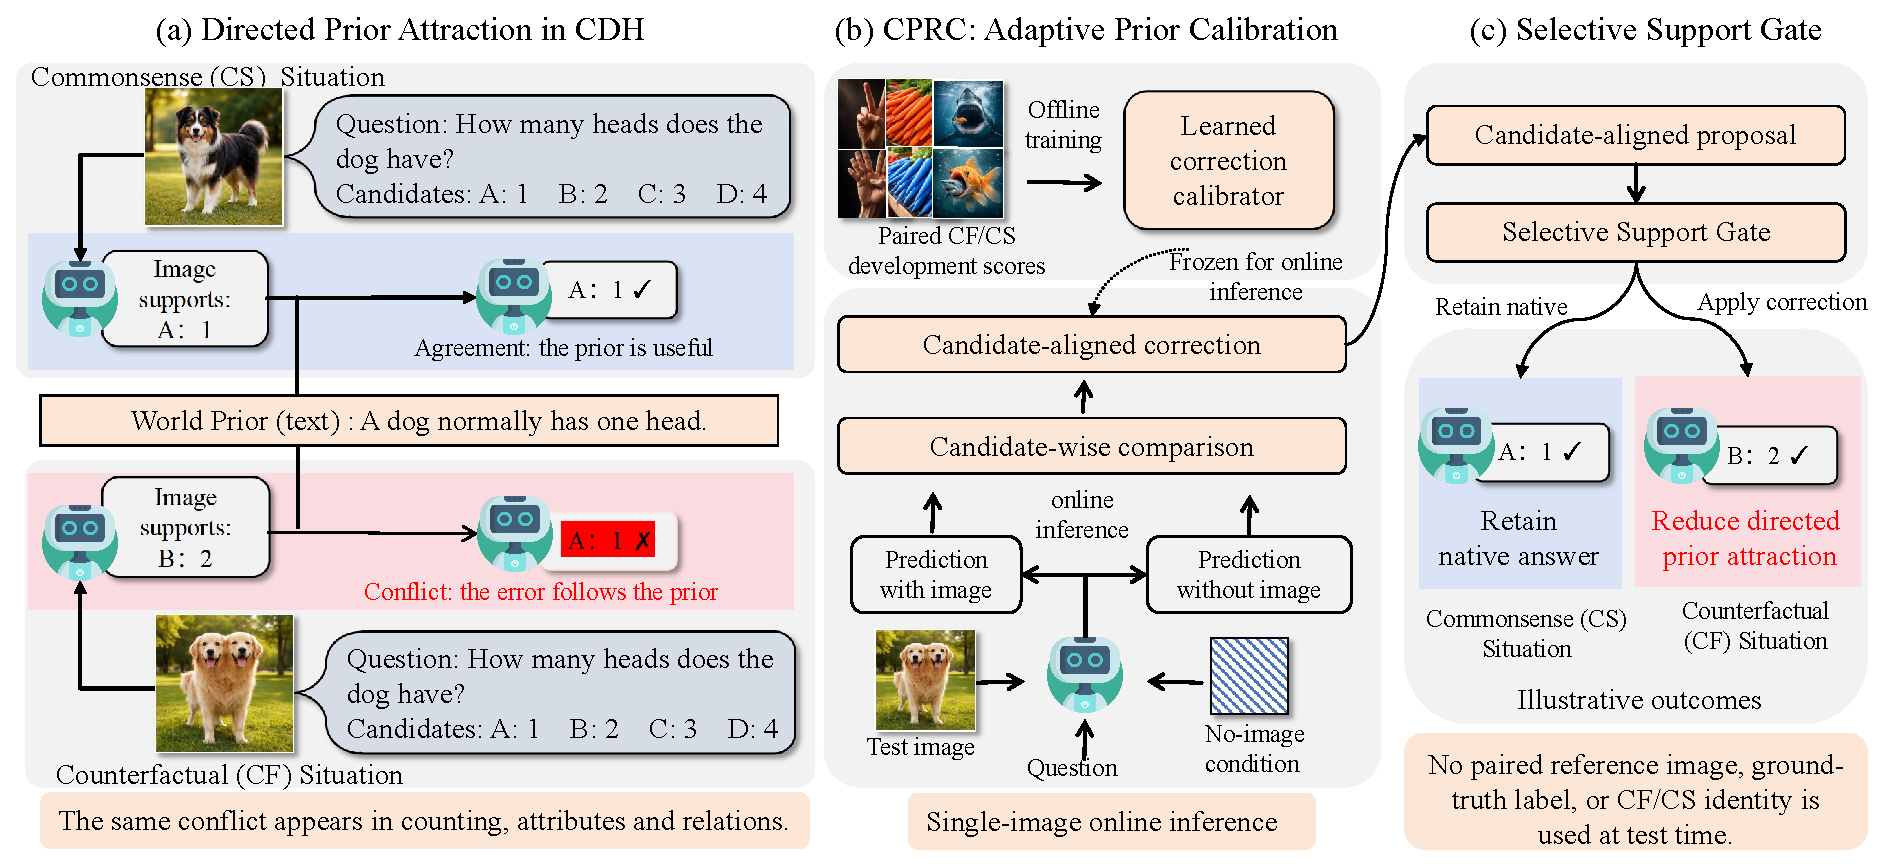
\includegraphics[width=0.90\textwidth]{figures/cdh_cprc_overview.pdf}
\caption{\textbf{From directed prior attraction to selective correction.}
(a) CS evidence agrees with the estimated world-prior preference, whereas the CF error is
pulled toward that same ordinary answer: \emph{directed prior attraction}.
(b) CPRC learns how much candidate-aligned prior preference to subtract and
proposes a correction from one test image. (c) The Selective Support Gate keeps
the native answer unless the score pattern supports that proposal. The matched
image, ground truth, and CF/CS side are unavailable at test time; the prior
sentence in (a) visualizes a prior-estimation score, not an extra input.}
\label{fig:overview}
\end{figure*}

Object-hallucination benchmarks evaluate unsupported objects, attributes, and
relations \cite{rohrbach2018chair,li2023pope,wang2023amber}, and a line of
interventions rescores, re-decodes, or re-attends the visual input
\cite{leng2024vcd,huang2024opera,chen2024halc,liu2024pai,wu2026revis}. Studies
of language bias and visual--knowledge arbitration examine related tensions
\cite{agrawal2018priors,zhou2025causalmm,liu2025insight,golovanevsky2025pixels},
without asking which specific answer replaces the visual one. Most closely,
NoLan dynamically contrasts multimodal and text-only token
distributions to suppress language priors in object hallucination
\cite{ren2026nolan}. CDH \cite{chen2026cdh} asks a different decision question:
which familiar answer overrides visible atypical evidence, and how can it be
weakened without losing that same answer when it is visually correct?

The paired CDH benchmark
\cite{chen2026cdh} provides a precise testbed for this question. Each concept appears as a counterfactual (CF) image, where
visual evidence conflicts with common sense, and a matched commonsense (CS)
control image, where visual evidence and world knowledge support the same
answer. That work measured the CF--CS gap; here we identify the candidate that
attracts the errors and study selective correction. We first
locate the answer toward which errors move, then learn a selective correction
from paired experience, and finally evaluate its transfer and failure
conditions.

The paired conflict suggests looking for an answer-specific pull. REVIS and
NoLan show that suppressing visual information exposes a language/world prior
entangled with visual decisions \cite{wu2026revis,ren2026nolan}. We score the same candidate answers in
an image-conditioned pass and a matched prior-estimation pass. CDH errors do not
scatter among plausible outputs: when the image-conditioned model fails on a
CF image, its wrong answer is usually the candidate ranked first in the
prior-estimation condition. We call this candidate the normal-world competitor. The
same structure appears across counts, colors, materials, functions, physical
states, spatial and causal relations, and animal behavior, and it remains
visible when an entire semantic family is absent from calibration.

We call this pattern \emph{directed prior attraction}. A
harder case occurs when the native output and both score views all favor the
ordinary answer, but subtracting the estimated prior preference reveals another
candidate. We call this decision pattern \emph{prior absorption}: the visual
alternative is present in the score distribution but does not win until the
ordinary preference is reduced. Both terms are descriptive at the decision
level.

This diagnosis suggests a minimal intervention: subtract the current
question's estimated prior preference from its image-conditioned scores.
However, direct removal degrades ordinary scenes. On CS images, the same prior
is often useful, and a model can exploit it as a shortcut for familiar
questions instead of resolving all visual evidence. The paired benchmark thus
measures both sides of the problem: CF repair and the corresponding CS cost. CPRC addresses this tradeoff by extracting
image--prior conflict evidence, learning a feature-conditioned calibrator from
paired development experience, and retaining the native answer when the
corrected proposal is not supported by the candidate-score pattern. An
optional extension that adds a released analytic rule on abstained examples is
examined in the Discussion.

The paper connects diagnosis to correction through the first answer-specific
paired analysis of CDH. At test time, CPRC receives only the queried image. Paired
fitting and direction controls isolate what is corrected; semantic holdouts,
option permutations, and external conflict data show how far it generalizes;
existence benchmarks and QA rewrites mark its scope and failure conditions. To our knowledge, this is the first dedicated
mitigation study under the paired CDH repair--retention protocol.

\section{Paired CDH and Research Questions}

\paragraph{Terminology.} Three score-level terms recur: the \emph{normal-world
competitor} is the candidate ranked first under the prior-estimation condition;
\emph{directed prior attraction} is the convergence of native CF errors onto
that candidate; \emph{prior absorption} is the stricter pattern in which every
score view favors the ordinary answer, yet subtracting its preference promotes
another.

Before correcting CDH, we must distinguish visual recovery from a much easier
strategy: preferring whatever answer looks unusual. The paired contrast in
Fig.~\ref{fig:overview}(a) makes that distinction observable. In the illustrated
example, the same question is applied to a two-headed CF image and its
one-headed CS control; only the visually correct answer changes. The pair
jointly measures CF repair and any degradation on the matched CS control.

The benchmark contains 300 concepts, each shown in a CF and a CS state, across
14 counting, attribute, and relation subcategories. A model receives one image
at a time. Following the original CDH evaluation protocol
\cite{chen2026cdh}, for native baseline $b$ and mitigation $m$ we jointly
report
\begin{equation}
\Delta_{CF}=Acc^{m}_{CF}-Acc^{b}_{CF},\qquad
\Delta_{CS}=Acc^{m}_{CS}-Acc^{b}_{CS}.
\label{eq:deltas}
\end{equation}
CF recovery without CS retention can be achieved by blindly preferring unusual
answers, so every result includes both sides and repair/harm counts.

Multiple choice (MC) is the primary task: answer positions cover A--D and can
be permuted without changing semantics. Native binary QA uses an ordinary-first
contrast, such as ``Does the hand have five fingers and not six?'' This phrasing
makes most CF labels ``no'' and most CS labels ``yes,'' creating a strong answer
direction. We report QA as a diagnostic of the prior estimator and MC
as the direction-robust headline.

These observations lead to four questions that organize the experiments.
\textbf{RQ1} asks whether CDH errors move toward a specific prior-favored candidate.
\textbf{RQ2} asks whether subtracting that direction repairs CF while paired
calibration retains CS. \textbf{RQ3} tests whether the effect survives unseen
semantic families, data splits, option permutations, a third checkpoint, and
independent conflict benchmarks.
\textbf{RQ4} evaluates the scope of the correction: on existence questions not built
around a directed candidate-aligned competitor, and on QA rewrites whose estimated prior no longer tracks
the same ordinary claim.

\section{Candidate-Aligned Prior-Residual Calibration}

The two-headed dog gives the method in one sentence: lower the model's
preference for ``one head'' when the remaining candidate evidence
supports ``two.'' CPRC turns this idea into four steps (Fig.~\ref{fig:overview}):
score the current answers under visual evidence and a prior-estimation
condition, summarize their conflict, learn how strongly to subtract the prior
preference, and decide whether to use the corrected proposal. An optional
extension for abstained examples appears in the Discussion.

\subsection{Candidate-Level Prior Evidence and Correction}

Let $\mathcal{Y}$ be the answers already supplied by the task: A--D for MC and
yes/no for QA. The frozen large vision--language model (LVLM) first generates a
native answer $i_b$. We then teacher-force each complete answer key and sum its
token log-probabilities, obtaining an image-conditioned score $s_I(y)$.
Removing the image yields the prior-estimation score $s_P(y)$. All
primary experiments instantiate this condition by removing the image block.
Replacing the missing image with white, black, or development-mean inputs does
not improve CF repair under the frozen route, so we retain the missing-image
estimator (supplement).
We center each vector by subtracting its mean and write
$i_I=\arg\max_y\bar s_I(y)$ and $i_P=\arg\max_y\bar s_P(y)$. Centering removes
arbitrary score offsets, and permuting candidate indices leaves the decision
unchanged; prompt reordering may still alter the scorer, so RQ3 tests three
option permutations.

The prior-estimate winner $i_P$ identifies the competing answer, while a learned
coefficient controls how much of that preference to remove. For evidence
$o=(\bar s_I,\bar s_P,i_b,K)$ and candidate count $K$, the corrected score is
\begin{align}
u&=\phi(o),\qquad \lambda_\theta(o)=c_\theta(u),\nonumber\\
s_C(y)&=\bar s_I(y)-\lambda_\theta(o)\bar s_P(y).
\label{eq:cprc}
\end{align}
Here $\bar s_P$ is an answer-specific proxy for language and world knowledge.
The subtraction is candidate-aligned
because each candidate loses its own estimated prior preference rather than a shared
penalty. A fixed coefficient is the special case in which $c_\theta$ ignores
$u$; CPRC instead lets the amount of subtraction change with the observed
image--prior score pattern.

The closest score rule, NoLan \cite{ren2026nolan}, chooses
$\alpha(o)=\beta[\tanh(1/D_{\mathrm{SKL}}(q_I,q_P))+1]$ and ranks candidates by
$(1+\alpha)\bar s_I-\alpha\bar s_P$, where $q_I,q_P$ are the softmax
normalizations of $\bar s_I,\bar s_P$, $D_{\mathrm{SKL}}$ is their symmetrized
KL divergence, and $\beta=0.8$ is NoLan's released constant. Because positive rescaling does not change
the winner, this is Eq.~\ref{eq:cprc} with
$\lambda_N(o)=\alpha(o)/(1+\alpha(o))$. NoLan is therefore an important
hand-designed calibrator based on one divergence. CPRC learns the map from the
full score pattern using paired CF/CS evidence and places a support decision
after the proposal; the subtraction direction itself is shared.

\paragraph{Why candidate alignment changes the right margin.}
The correction should enlarge the margin against the ordinary answer rather
than perturb every alternative equally. Let \(y^*\) be the visually supported
answer, \(y\) one competitor, and \(\lambda=\lambda_\theta(o)\). Subtraction
changes their margin by
\begin{equation}
\bigl[s_C(y^*)-s_C(y)\bigr]
-\bigl[\bar s_I(y^*)-\bar s_I(y)\bigr]
=\lambda\bigl[\bar s_P(y)-\bar s_P(y^*)\bigr].
\label{eq:margin-shift}
\end{equation}
If the prior estimate prefers the wrong ordinary answer \(y\), positive
\(\lambda\) moves this margin toward vision. Mean, cross-question, or permuted
priors lose that sign guarantee; if the prior correctly favors \(y^*\),
subtraction can instead hurt. Candidate alignment supplies the direction,
while paired CS examples control its strength.

\subsection{Conflict Features and Prior Calibration}

Candidate alignment determines the subtraction direction; the calibrator
determines its magnitude.
The feature map $u=\phi(o)$ summarizes the two views' confidence, their
disagreement, and their agreement with the native output. Our experiments use a compact
13-dimensional instantiation built from the two distributions' entropies,
maxima, and top-two margins, their Jensen--Shannon divergence, and winner
indicators (full definition and per-term description in the supplement).

With only 70 development pairs, we use a capped linear--softplus calibrator,
$c_\theta(u)=\min\{\operatorname{softplus}(u^\top\theta),\lambda_{\max}\}$,
with Gaussian prior $\theta\sim\mathcal N(0,\rho^{-1}I)$. Its
maximum-a-posteriori (MAP) estimate minimizes the paired corrected-score loss
\begin{align}
\ell_i(\theta)&=-\log\!\left[
\operatorname{softmax}(\bar s_{I,i}-
\lambda_\theta(o_i)\bar s_{P,i})\right]_{y_i},\nonumber\\
\hat\theta&=\arg\min_\theta\sum_{i\in D}\ell_i(\theta)
+\frac{\rho}{2}\|\theta\|_2^2.
\label{eq:fit}
\end{align}
where $D$ is the set of development rows and $y_i$ the correct answer of row
$i$. For the two full-matrix checkpoints, one calibrator is fitted jointly across MC
and QA: each development pair contributes its CF and CS row in both formats.
Joint fitting on CF and CS rows estimates the correction strength while
limiting overcorrection on ordinary cases. We select regularization and the output
cap by maximizing the mean task utility $\Delta CF+0.5\Delta CS$, subject to
nonnegative CF change and at most four percentage points of CS loss in each
format. No task or category label enters $u$. The selected values are then used
without test-set retuning; the search grid is reported in the supplement.
A margin-level condition for when this correction provably recovers the
visually supported answer, and a measured stability analysis of the fitted
coefficients, appear in the supplement.

\subsection{Selective Decision and Inference}

Mitigation also requires deciding whether to override the native answer. On either side the
accuracy change is exactly the number of repairs minus harms, normalized: an
accepted override either fixes a wrong native answer or breaks a correct one.
With only 70 pairs, we use a low-capacity structural gate instead of a
learned correctness predictor: CPRC separates the learned
proposal in Eq.~\ref{eq:cprc} from a small Selective Support Gate, and a
four-percentage-point CS budget decides how much harm to tolerate at the
dataset level.

\paragraph{The learned route.}
The learned route proposes
$z_M=\arg\max_y s_C(y)$ using $\hat\theta$. It accepts a non-native proposal in
two interpretable cases seen during calibration. In \emph{direct conflict},
$i_I\ne i_P$ and correction selects the image-score winner $z_M=i_I$. In
\emph{prior absorption}, $i_b=i_I=i_P$ but subtracting the strong estimated
prior preference reveals a different candidate $z_M$; this is the operational pattern
defined in the Introduction. The candidate count must also fall within the
development range, and the corrected top-two margin must exceed a
development-fitted threshold (Algorithm~\ref{alg:gate}). Otherwise the Gate keeps the native answer. These criteria
use only score structure.

\begin{algorithm}[t]
\caption{Selective Support Gate (learned route).}
\label{alg:gate}
{\footnotesize
\begin{tabular}{@{}r@{\enskip}p{0.82\columnwidth}@{}}
\multicolumn{2}{@{}p{0.9\columnwidth}@{}}{\textbf{Input:} native answer $i_b$; corrected scores
$s_C$ at $\lambda_{\hat\theta}(o)$; score-view winners $i_I,i_P$; corrected
top-two softmax margin $m$; candidate count $K$; threshold $m_{\min}$.}\\[3pt]
1: & $z_M \gets \arg\max_y s_C(y)$\\
2: & $\mathit{conflict} \gets (i_I \ne i_P) \land (z_M = i_I)$\\
3: & $\mathit{absorption} \gets (i_b = i_I = i_P) \land (z_M \ne i_b)$\\
4: & $g_M \gets [z_M \ne i_b] \land [K\ \textrm{in development range}]
\land [m \ge m_{\min}] \land (\mathit{conflict} \lor \mathit{absorption})$\\
5: & \textbf{return} $z_M$ \textbf{if} $g_M=1$, \textbf{else} $i_b$\\
\end{tabular}}
\end{algorithm}

\paragraph{Optional analytic coverage (CPRC+NoLan).}
A conservative learned gate can miss valid corrections that a simpler
prior-residual rule reaches. An optional extension, \textbf{CPRC+NoLan},
therefore evaluates NoLan's released analytic proposal on rows the learned
route keeps, and adopts it whenever it differs from the native answer. The
learned route keeps precedence wherever its gate accepts, so no supported
learned correction is displaced, and both proposals reuse the same scores, so
the extension adds no LVLM forward pass. The learned route alone is
\textbf{CPRC}, the primary method. The extension's decision rule, a posterior
gate variant, and the relaxed-budget \emph{High-Repair} operating point used
for attribution diagnostics appear in the supplement.

\section{Experimental Setup}

\paragraph{Inference boundary.}
At test time, each method receives one image, the native question, and the
task-native candidate set. Paired images, CF/CS identities, semantic
categories, and test labels enter development and evaluation only.

\paragraph{Data and models.}
We reserve five pairs from each of the 14 subcategories (70 pairs) for fitting
and model selection, and evaluate the remaining 230 unseen concepts.
Qwen3-VL-32B \cite{bai2025qwen3vl} and LLaVA-1.6-34B
\cite{liu2024llavabaselines} are evaluated on both MC and QA. A third checkpoint,
Qwen3-VL-30B-A3B, provides an MC replication with a sparse language decoder and
the same 70/230 split.

\paragraph{Baselines and matched controls.}
We compare Focus-on-Vision-style grounding \cite{liu2025insight}, VCD
\cite{leng2024vcd}, MFCD \cite{liu2025mfcd}, PAI \cite{liu2024pai}, NoLan
\cite{ren2026nolan}, and official REVIS \cite{wu2026revis}. VCD, MFCD, and PAI
replay their published score equations over native candidates. NoLan applies its
released dynamic rule to complete-answer distributions, which we evaluate as a
score rule. REVIS uses its released latent
intervention and family coefficient. Tunable methods share the 70 pairs,
objective, and four-point development CS budget; fixed methods keep released
settings. CPRC+NoLan reuses NoLan's released coefficient only for its analytic
fallback; the standalone NoLan row applies that rule to every example. Matched
controls use CPRC's gate with a constant coefficient, train a
logistic gate for fixed-residual proposals, or pass PAI proposals through that
gate, separating calibration, proposal direction, and acceptance capacity.

All methods operate on the task's original output space: MC scores A--D and QA
scores yes/no under the native question. No task reformulation, candidate hint,
or supplementary answer information is introduced. Each selected configuration
is fixed on development data before the shared test evaluation. A
format-specific variant fitted on development MC alone transfers at least as
well to held-out MC as the joint fit
(supplement), so the joint
MC+QA fit mainly adds QA coverage.

\paragraph{Robustness, transfer, and statistics.}
Three option permutations test position dependence. The QA stress test asks
the same ordinary and atypical claims in both orders, using one fitted wording
and three unseen templates. We also refit ten stratified splits, use as few as
14 development pairs, and remove each of the three broad semantic families.
Primary transfer uses the same four-point learned route on every external
benchmark: 1,220 Visual
CounterFact pairs \cite{golovanevsky2025pixels}, HallusionBench
\cite{guan2024hallusionbench}, ConflictVIS \cite{liu2025insight}, and two
existence benchmarks, POPE \cite{li2023pope} and a 70-pair transfer set built
from official POPEv2 annotations (object-presence questions on paired
present/absent images).
A separately identified high-repair policy is used only for the RQ1 attribution
diagnostics. We
report repair/harm counts, exact paired McNemar tests, and 10,000 pair-level
bootstrap samples. Prompts, search grids, implementation details, and confidence
intervals are provided in the supplement.

\section{Results}

RQ1 locates the candidate that attracts CDH errors; RQ2 tests whether
subtracting it repairs CF while retaining CS; RQ3 evaluates generalization;
and RQ4 evaluates scope. Figure~\ref{fig:evidence-chain}
summarizes the direction controls and the repair--retention frontier, while
Tables~\ref{tab:spectrum} and~\ref{tab:equivariance}
report the two boundaries.

\subsection{RQ1: CDH Errors Follow a Specific Prior}

If CDH is a candidate-aligned pull from ordinary-world knowledge, native CF
errors should repeatedly land on the prior-estimate winner, and candidate
shuffling should destroy repair.

\begin{figure*}[t]
\centering
\begin{minipage}[b]{0.64\textwidth}
\centering
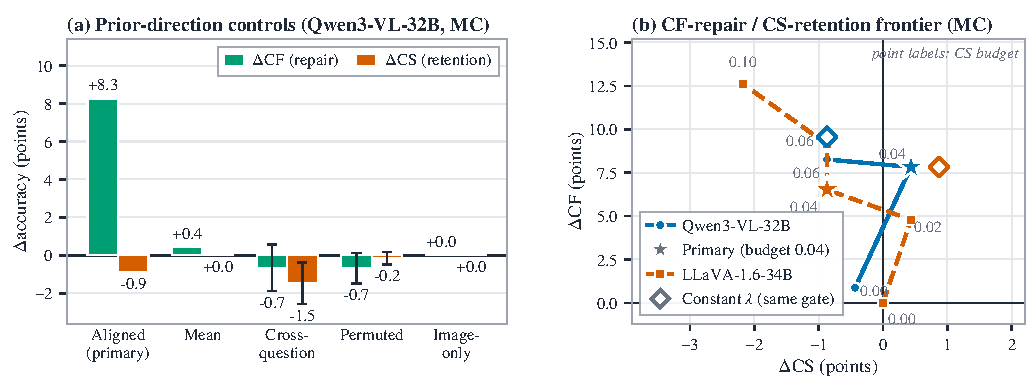
\includegraphics[width=\linewidth]{figures/evidence_chain_v2.pdf}
\caption{\textbf{Direction controls and the repair--retention frontier (MC).}
(a) At the frozen High-Repair attribution point (Qwen3-VL-32B, MC), the aligned
prior residual repairs $+8.3$ CF points for a $0.9$-point CS loss, while
replacing the current prior by the development mean, another question's prior,
or a candidate permutation removes nearly all gain ($-0.7$ to $+0.4$ CF); an
image-only residual changes nothing. Error bars show the standard deviation
across seeds. (b) The learned route traces the CF-repair/CS-retention
frontier on both models as the development CS budget varies (point labels);
stars mark the primary operating point (budget $0.04$) and open diamonds the
matched constant-coefficient control.}
\label{fig:evidence-chain}
\end{minipage}\hfill
\begin{minipage}[b]{0.34\textwidth}
\centering
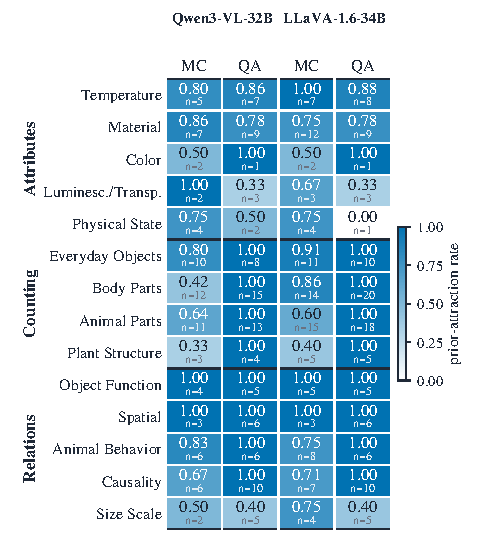
\includegraphics[width=\linewidth]{figures/rq1_subcategory_matrix.pdf}
\caption{\textbf{Directed prior attraction by subcategory.} Fraction of native
counterfactual errors whose answer equals the prior-estimate winner, per model
and format; cell annotations give the error count $n$.}
\label{fig:rq1-matrix}
\end{minipage}
\end{figure*}

Among native CF errors, the wrong answer equals the prior-estimate winner in 70.1\%
of Qwen MC cases and 90.4\% of its QA cases; the corresponding LLaVA rates are
77.0\% and 91.6\%. In 80.5--91.6\% of these
errors, that winner is also the correct answer on the paired CS image. The
third checkpoint shows the same pattern: 68 of 84 MC errors select the prior-estimate
winner, which is the CS answer in 76 cases. The error distribution is
concentrated on a concrete normal-world answer.
Figure~\ref{fig:rq1-matrix} breaks this convergence down by subcategory:
attraction is near-saturated for counting and relational QA errors and weaker
for attribute anomalies and MC counting errors (several attribute cells contain
at most three errors).

The controls isolate what matters about that direction. Replacing each prior by
the development mean, borrowing one from another question with the same number
of answers, or permuting its candidate values removes nearly all MC gain
(Fig.~\ref{fig:evidence-chain}(a)). On Qwen MC, the aligned residual gains 8.3 CF
points for a 0.9-point CS loss; the three replacements range from a 0.7-point
loss to a 0.4-point gain. An image-only residual produces no change. Because
each replacement is refitted with the same data and gate, the result identifies
the current question's candidate alignment as the useful correction direction. This diagnostic suite uses the already
frozen secondary High-Repair point so every direction control is compared under
one jointly selected operating point.

At $\lambda=0$, teacher-forced image scoring changes CF accuracy
by -22.6 to -0.9 points across the four model--format cells, so the gain comes
from the aligned prior residual.

\subsection{RQ2: A Minimal Residual Repairs CF While Retaining CS}

RQ2 tests whether subtracting the identified preference creates a useful
decision rather than another shortcut. MC is the direction-robust setting
because its answer positions can be permuted; every gain
is read beside matched CS retention and repair/harm counts.

\begin{table*}[t]
\centering
\small
\begin{tabular*}{\textwidth}{@{\extracolsep{\fill}}lrrrrrr@{}}
\toprule
Model & Native CF & Native CS & $\Delta$CF [95\% CI] & $\Delta$CS [95\% CI]
& CF R/H & CS R/H \\
\midrule
Qwen3-VL-32B
& 0.665 & 0.965 & +7.8 [3.9, 12.2] & +0.4 [-2.2, 3.0] & 21/3 & 5/4 \\
LLaVA-1.6-34B
& 0.565 & 0.917 & +7.0 [3.5, 10.4] & -0.4 [-2.6, 1.7] & 17/1 & 3/4 \\
\bottomrule
\end{tabular*}
\caption{Primary CPRC results on 230 unseen MC pairs. Changes are accuracy
points and intervals use 10,000 pair-level bootstrap samples. R/H is the
number of repaired/harmed predictions.}
\label{tab:main}
\end{table*}

\begin{table}[!tb]
\centering
\footnotesize
\setlength{\tabcolsep}{1.4pt}
{\scriptsize
\begin{tabular*}{\columnwidth}{@{\extracolsep{\fill}}lrrrr@{}}
\toprule
Method & Qwen MC & Qwen QA & LLaVA MC & LLaVA QA \\
\midrule
Focus on Vision & -0.9/+0.4 & +8.7/-0.4 & -12.6/+3.0 & -13.0/+2.2 \\
VCD & +4.4/-2.2 & -1.3/+0.0 & -2.2/-2.6 & -2.2/-0.4 \\
MFCD & +3.5/-2.2 & -1.3/+0.0 & +2.6/-0.4 & +5.2/-0.9 \\
PAI & +0.9/-0.9 & -17.8/-0.4 & +6.5/+0.9 & +21.3/-4.3 \\
REVIS & -1.3/+0.0 & -2.2/-0.4 & -1.3/+0.9 & +14.8/-3.0 \\
NoLan score rule & \textbf{+10.0/-0.4} & +6.5/+0.0 & \textbf{+7.8/+0.4} & \textbf{+27.0/-6.1} \\
\midrule
CPRC (ours) & +7.8/+0.4 & \textbf{+22.2/-1.7} & \textbf{+7.0/-0.4} & \textbf{+23.9/-4.8} \\
CPRC+NoLan (ours) & \textbf{+9.6/-0.4} & \textbf{+22.2/-1.7} & \textbf{+8.3/-0.4} & \textbf{+27.0/-6.1} \\
\bottomrule
\end{tabular*}}
\caption{Baseline comparisons in accuracy points ($\Delta$CF/$\Delta$CS
relative to native). Tunable rows use the same development split, utility, and
per-task four-point CS budget; NoLan and REVIS keep released settings. The
NoLan row serves both as a strong external analytic baseline and as an
independent validation of candidate-aligned prior subtraction. Bold marks the
leading prior-subtraction rows in each model--format cell.}
\label{tab:controlled}
\end{table}


At the primary setting (Table~\ref{tab:main}), the learned route gains
substantially on CF for a near-zero CS change. Figure
\ref{fig:evidence-chain}(b) shows the underlying learned-route frontier; the
selected point spends almost none of the CS budget.

\begin{table}[!b]
\centering
\small
\setlength{\tabcolsep}{2.5pt}
\begin{tabular*}{\columnwidth}{@{\extracolsep{\fill}}lrr@{}}
\toprule
Fit / selection & MC & QA \\
\midrule
\multicolumn{3}{l}{\itshape Qwen3-VL-32B} \\
Both / both & +7.8/+0.4 & +22.2/-1.7 \\
Both / CF only & +8.3/-0.9 & +23.9/-4.3 \\
CF only / CF only & +9.6/-58.7 & +34.4/-83.0 \\
\midrule
\multicolumn{3}{l}{\itshape LLaVA-1.6-34B} \\
Both / both & +7.0/-0.4 & +23.9/-4.8 \\
Both / CF only & +12.2/-1.3 & +30.0/-9.6 \\
CF only / CF only & +17.0/-38.3 & +40.9/-79.6 \\
\bottomrule
\end{tabular*}
\caption{Why both sides of the pair are needed. Each cell reports
$\Delta$CF/$\Delta$CS in accuracy points. ``Both'' means CF and CS; the two
parts of the first column name the fitting data and trade-off selection data.}
\label{tab:paired-calibration}
\end{table}

Paired fitting and paired selection play different roles
(Table~\ref{tab:paired-calibration}). Selecting for CF alone spends more CS even
when the fit has seen both sides. Removing CS from the fit is far more damaging:
the calibrator becomes an almost unconditional answer changer, losing
38.3--83.0 CS points. Both CF and CS rows are therefore required during
calibration.

Table~\ref{tab:controlled} separates correction direction from decision
coverage. NoLan independently confirms that dynamic prior subtraction reaches
CDH; on MC it matches or exceeds the learned route in distribution. The largest
difference appears on Qwen QA, where the learned route adds 36 net CF repairs
over the analytic rule (exact McNemar
$p=2.9\times10^{-11}$) at no significant CS cost, and under distribution shift
the adaptive routes exceed the fixed-coefficient control by 1.1--3.2 utility
points across the semantic-holdout and 14-pair settings (supplement). A
constant coefficient is likewise competitive on in-distribution MC (20 of 460
test decisions differ from the learned route, $p=1.0$) but trails it on QA.
Matched controls that share the development data and score features, including
a calibrator fitted on development MC alone, appear in the supplement.

The Gate mainly controls retention; gate deletions, coefficient
distributions, and 14-pair refits appear in the supplement.

\subsection{RQ3: The Correction Generalizes}

An in-distribution gain could still reflect familiar counts, templates, or
option positions. We move away from the original fit in stages:
exclude whole semantic families, refit independent splits with fewer examples,
permute answer positions, and finally evaluate a CDH-selected policy on
independent data.

The 14 subcategories form three broad families: attributes, counting, and
relations. Leaving any one family out of fitting still produces positive CF
change in every model/task cell for the learned route. Qwen MC gains
9.3, 10.0, and 6.7 points on the three held-out families; LLaVA gains 5.3,
10.0, and 10.7 points. The third checkpoint also remains positive on CF, with
CS changes between a 5.3-point loss and a 1.3-point gain. The learned calibrator
thus generalizes across semantic ranges without receiving a category label.

All 40 learned-route outcomes across ten stratified refits improve CF; mean MC changes are
+7.6/-0.8 for Qwen and +10.0/-2.1 for LLaVA. Three option permutations retain
5.2--7.8 and 12.6--13.9 CF points, with absolute CF accuracy varying by at most
2.2 points. The gain is not tied to one split or answer position.

Visual CounterFact independently reproduces the signature: 45 of 46 Qwen
errors and all 75 LLaVA errors select the prior-estimate winner, which is always the
ordinary attribute. The learned route, fitted only on CDH, transfers
at +3.11/-0.25 points for Qwen and +4.51/-0.08 for LLaVA.
This is the primary external result.

The same frozen policy transfers to two further conflict benchmarks.
HallusionBench gains +5.2 CF points for a 0.9-point CS loss (McNemar
$p=4.9\times10^{-4}$), compared with +0.61/-0.91 for official REVIS, and
ConflictVIS gains +2.1 MC points (8 repairs, no harms, $p=0.008$) and +25.7
points on its yes/no subset, whose labels are all yes and which therefore
is reported as supporting evidence only.

\subsection{RQ4: Scope and Failure Conditions}

RQ3 shows that the correction generalizes; the last question is its scope.
The first boundary is the task itself. Table~\ref{tab:spectrum} evaluates one
frozen operating point across six benchmarks: four carry a directed
normal-world competitor, and two probe object existence, which is not
constructed around a specific candidate-aligned competitor.

\begin{table*}[t]
\centering
\footnotesize
\setlength{\tabcolsep}{2.0pt}
{\scriptsize
\begin{tabular*}{\textwidth}{@{\extracolsep{\fill}}llr rr c rr c rr c@{}}
\toprule
 & & & \multicolumn{3}{c}{CPRC (ours)} & \multicolumn{3}{c}{CPRC+NoLan (ours)} & \multicolumn{3}{c}{NoLan} \\
\cmidrule(lr){4-6} \cmidrule(lr){7-9} \cmidrule(lr){10-12}
Benchmark & Type & $N$ & int. & rep./harm & $\Delta$CF/$\Delta$CS & int. & rep./harm & $\Delta$CF/$\Delta$CS & int. & rep./harm & $\Delta$CF/$\Delta$CS \\
\midrule
CDH MC (held-out) & conflict (in-dist.) & 460 & 40 & 26/7 & +7.8/+0.4 & 50 & 31/10 & +9.6/-0.4 & 48 & 31/9 & +10.0/-0.4 \\
CDH QA (held-out) & conflict (in-dist.) & 460 & 59 & 53/6 & +22.2/-1.7 & 59 & 53/6 & +22.2/-1.7 & 19 & 17/2 & +6.5/+0.0 \\
Visual CounterFact & conflict (transfer) & 2440 & 45 & 40/5 & +3.1/-0.2 & 46 & 41/5 & +3.2/-0.2 & 38 & 36/2 & +2.9/-0.1 \\
HallusionBench & illusion conflict (transfer) & 656 & 34 & 24/10 & +5.2/-0.9 & 122 & 66/56 & +6.7/-3.7 & 109 & 57/52 & +4.3/-2.7 \\
ConflictVIS MC & conflict (transfer) & 374 & 8 & 8/0 & +2.1 & 8 & 8/0 & +2.1 & 8 & 8/0 & +2.1 \\
ConflictVIS QA & conflict (transfer) & 374 & 96 & 96/0 & +25.7 & 97 & 97/0 & +25.9 & 97 & 97/0 & +25.9 \\
\shadedrow POPE & existence & 9000 & 17 & 6/11 & -0.1/+0.0 & 864 & 387/477 & -1.0/+0.0 & 864 & 387/477 & -1.0/+0.0 \\
\shadedrow POPEv2 & existence (transfer) & 140 & 1 & 0/1 & -1.4/+0.0 & 23 & 0/23 & -32.9/+0.0 & 23 & 0/23 & -32.9/+0.0 \\
\bottomrule
\end{tabular*}}
\caption{Benchmark spectrum under one frozen operating point, all with
Qwen3-VL-32B; LLaVA-1.6-34B transfers to Visual CounterFact
at +4.5/-0.1. Interventions (int.) count
non-native final answers; rep./harm counts repairs and harms against gold;
deltas are accuracy points relative to native. The delta pair reads
$\Delta$CF/$\Delta$CS for the CDH, Visual CounterFact, and HallusionBench
rows, $\Delta$Accuracy/$\Delta$F1 for POPE, $\Delta$absent/$\Delta$present
for POPEv2, and $\Delta$Accuracy for ConflictVIS. Shaded rows are existence benchmarks: CPRC repairs
where a directed normal-world competitor exists and changes few
predictions, without significant cost, where that structure is absent.}
\label{tab:spectrum}
\end{table*}

On the existence side, CPRC intervenes on 17 of 9,000 POPE
questions and 1 of 140 POPEv2 questions, with no significant accuracy change
($p=0.33$ and $p=1.0$). The correction thus has a measurable scope: it
intervenes where a directed normal-world competitor exists and changes few
predictions where that structure is absent. The extension columns quantify what that
selectivity is worth (Discussion).

The second boundary is semantic. Within conflict tasks, the correction
improves both answer directions only while the estimated prior still denotes
the same ordinary claim.
Consider ``Does the hand have five fingers rather than six?'' and its
swap, ``Does the hand have six fingers rather than five?'' A prior that truly
favors the ordinary five-finger claim should answer yes to the first wording and
no to the second. A fixed yes/no bias will not make that change. We use these
meaning-preserving swaps to separate the two cases. Native QA averages also
hide a strong directional skew: on the original CF wording,
Qwen and LLaVA gain 26.1 and 32.6 points among 218 ``no'' answers, but each
loses 16.7 points among the 12 ``yes'' answers, so the same semantic claims
must be tested in both orders.

We call a pair \emph{meaning-aligned} when the prior-estimation pass favors the ordinary
claim in both orders: yes for ordinary-first and no for atypical-first. This
partition uses the benchmark's ordinary/atypical roles only for analysis; CPRC
never sees them. Table~\ref{tab:equivariance}
reports both CF repair and the accompanying CS change within each group.

\begin{table}[!tb]
\centering
\footnotesize
\setlength{\tabcolsep}{2.5pt}
{\scriptsize
\begin{tabular*}{\columnwidth}{@{\extracolsep{\fill}}lrr@{}}
\toprule
Template & Meaning-aligned & Other \\
\midrule
\multicolumn{3}{l}{\itshape Qwen3-VL-32B} \\
Contrastive & 132; +46.2/+22.7; -3.8 & 98; +22.4/-3.1; -1.5 \\
Instead & 106; +25.5/+21.7; -0.5 & 124; +9.7/+0.0; +0.0 \\
Choice & 113; +8.0/+23.0; +0.0 & 117; -1.7/-0.9; +0.9 \\
Reject-second & 56; +55.4/+26.8; -0.9 & 174; +44.3/-6.3; +0.3 \\
\midrule
\multicolumn{3}{l}{\itshape LLaVA-1.6-34B} \\
Contrastive & 107; +52.3/+14.0; -4.7 & 123; +41.5/-14.6; -1.2 \\
Instead & 33; +60.6/+9.1; -1.5 & 197; +56.3/-14.7; -4.6 \\
Choice & 13; +23.1/+7.7; -11.5 & 217; +21.2/-15.2; -2.5 \\
Reject-second & 0; --; -- & 230; +82.2/-43.0; +17.0 \\
\bottomrule
\end{tabular*}}
\caption{QA boundary analysis on 230 unseen pairs per template. Each cell gives
$N$; $\Delta$CF for ordinary-/atypical-first wording; pooled $\Delta$CS (points).}
\label{tab:equivariance}
\end{table}

Every nonempty meaning-aligned group improves CF in both directions and contains
no CF harms. Pair-bootstrap intervals remain nonnegative, although the
13-example LLaVA Choice group is necessarily wide ([0.0, 34.6]). When alignment
fails, the atypical-first direction is nonpositive for Qwen and loses
14.6--43.0 points for LLaVA. LLaVA's aligned count falls from 107 on the fitted
wording to 33, 13, and 0 on the unseen templates. A score-confidence gate cannot
recover a semantic competitor that the prior estimate no longer represents.

On the fitted wording, complementary and joint CF accuracy (defined in the
supplement) rise from 0.761/0.448
to 0.917/0.765 for Qwen and from 0.600/0.304 to 0.800/0.630 for LLaVA. Six of
eight Qwen CF comparisons remain significant after Holm adjustment over 32
model--template--order--side endpoints. QA is thus a strong diagnostic,
while MC remains the cleaner direction-robust result. Candidate length is not
an explanation: within each model, sum- and mean-normalized scoring give the
same fixed-residual predictions.

\section{Discussion and Conclusion}

The prior-estimate distribution identifies the competing normal-world answer, and
paired CS controls show when it remains useful: the correction is most
active when the estimated prior strongly favors a competing candidate. On
existence benchmarks without the directed-competitor structure, the gate
changes few predictions at no cost; within conflict tasks, the correction
improves both answer directions only while the estimated prior still denotes
the same ordinary claim.

An optional extension, CPRC+NoLan, adds NoLan's released analytic proposal
where the learned gate abstains. Decomposing all 1,840 held-out test rows by
proposal state shows that the two routes never disagree on a destination (the
conflict state is empty; supplement), so the extension
only fills abstentions, adding 16 CF repairs against 2 harms and raising MC CF
recovery to +9.6 and +8.3 points. Its cost appears where that competitor
structure is absent: on existence benchmarks the extension reduces to the ungated rule (864
POPE interventions, $-1.0$ point; 23 POPEv2 interventions, all harms). We
therefore evaluate CPRC+NoLan as a conflict-set option and keep CPRC as the
primary method.

The present realization assumes finite candidates,
checkpoint-level calibration, and one no-image prior-estimation pass;
open generation remains future work.

CDH occurs when visible atypical evidence loses to an ordinary answer that still
helps on matched CS images. CPRC estimates that competitor, learns a paired
candidate-aligned correction, and optionally extends it with the released
analytic proposal on abstained rows. The correction transfers across decoder
structures, semantic holdouts, option permutations, and independent conflict
data under frozen per-model operating points, and changes few
predictions on
existence benchmarks at no significant cost. CPRC is therefore a conflict-selective
correction with a measurable scope: it calibrates useful
world knowledge where that knowledge overrides vision, and largely preserves
native behavior elsewhere.

\bibliography{references}

\end{document}
